The Terminal API provides functions for sending text to the terminals, and drawing text-mode graphics. The API expects connected terminal to use Codepage 437. See section \emph{Codepage} for details.

\section{Functions}

Note: cursor coordinates starts from one, not zero.

\begin{tabularx}{\textwidth}{l l X}
	\textbf{\large Function} & \textbf{\large Return} & \textbf{\large Description}
	\\ \\
	\endhead
	term.write(string) & nil & Writes string to the current cursor position. Line feed is not appended.
	\\ \\
	term.print(string) & nil & Writes string to the current cursor position and make a new line.
	\\ \\
	term.newLine() & nil & Make a new line.
	\\ \\
	term.moveCursor(\textbf{x}: int) & nil & Moves cursor horizontally, starting from 1.
	\\ \\
	term.width() & int & Returns the width of the terminal. Graphic terminals also can use this.
	\\ \\
	term.scroll(\textbf{n}: int) & nil & Make a new line \textbf{n} times.
	\\ \\
	term.bell(pattern: string) & nil & Strikes a bell. Go to section \emph{Lua Globals} > \emph{Bell Codes} for accepted patterns.
	\\ \\
	term.isTeletype() & bool & Returns \textbf{true} if the terminal is teletype.
	\\ \\
	\multicolumn{3}{c}{\textbf{Graphic terminals only}}
	\\ \\
	term.emit(\textbf{c}: int, \textbf{x}: int, \textbf{y}: int) & nil & Emits \textbf{c} into (\textbf{x}, \textbf{y}), control sequence will not be processed and printed as symbols instead. Cursor will not be moved.
	\\ \\
	term.emitRaw(\textbf{bufferChar}: int) & nil & Emits \textbf{bufferChar} into into (\textbf{x}, \textbf{y}). Buffer char means a single character actually stored into the screen buffer, has four bits for back- and foreground colours respectively, and eight bits for a letter.
	\\ \\
	term.emitString(\textbf{s}, \textbf{x}: int, \textbf{y}: int) & nil & Emits \textbf{s} (a string) into (\textbf{x}, \textbf{y}), printing control sequences as symbols. Cursor will not be moved.
	\\ \\
	\begin{tabular}[t]{@{}l@{}}term.resetColour()\\term.resetColor()\end{tabular} & nil & Resets any colour changes to the defaults.
	\\ \\
	term.clear() & nil & Clears whole screen buffer and move cursor to (1, 1)
	\\ \\
	term.clearLine() & nil & Clears current line on the screen buffer, does not moves cursor.
	\\ \\
	term.setCursor(\textbf{x}: int, \textbf{y}: int) & nil & Moves cursor to (\textbf{x}, \textbf{y})
	\\ \\
	term.getCursor() & int, int & Returns current coordinates of the cursor.
	\\ \\
	term.getX() & int & Returns X coordinate of the cursor.
	\\ \\
	term.getY() & int & Returns Y coordinate of the cursor.
	\\ \\
	term.setX(int) & nil & Sets X coordinate of the cursor.
	\\ \\
	term.setY(int) & nil & Sets Y coordinate of the cursor.
	\\ \\
	term.setCursorBlink(bool) & nil & Sets cursor blinking. \textbf{true} makes the cursor blink.
	\\ \\
	term.size() & int, int & Returns width and height of the terminal.
	\\ \\
	term.height() & int & Returns height of the terminal. 
	\\ \\
	term.isCol() & bool & Returns if the terminal supports colour.
	\\ \\
	term.setForeCol(\textbf{col}: int) & nil & Sets foreground colour to \textbf{col}
	\\ \\
	term.setBackCol(\textbf{col}: int) & nil & Sets background colour to \textbf{col}.
	\\ \\
	term.foreCol() & int & Returns current foreground colour.
	\\ \\
	term.backCol() & int & Returns current background colour.
\end{tabularx}

\section{Standard Colours}

\begin{tabularx}{\textwidth}{c l c l c l c l}
	0 & \textcolor{black}{Black} & 1 & White & 2 & \textcolor{dimgrey}{Dim grey} & 3 & \textcolor{brightgrey}{Bright grey}
	\\ \\
	4 & \textcolor{yellow}{Yellow} & 5 & \textcolor{orange}{Orange} & 6 & \textcolor{red}{Red} & 7 & \textcolor{magenta}{Magenta}
	\\ \\
	8 & \textcolor{purple}{Purple} & 9 & \textcolor{blue}{Blue} & 10 & \textcolor{cyan}{Cyan} & 11 & \textcolor{lime}{Lime}
	\\ \\
	12 & \textcolor{green}{Green} & 13 & \textcolor{darkgreen}{Dark green} & 14 & \textcolor{brown}{Brown} & 15 & \textcolor{tan}{Tan}
\end{tabularx}

Non-colour terminals support colour index of 0--3.

\section{Codepage}

\newlength{\cpimagew}
\setlength{\cpimagew}{\linewidth}
\addtolength{\cpimagew}{-4em}

\begin{center}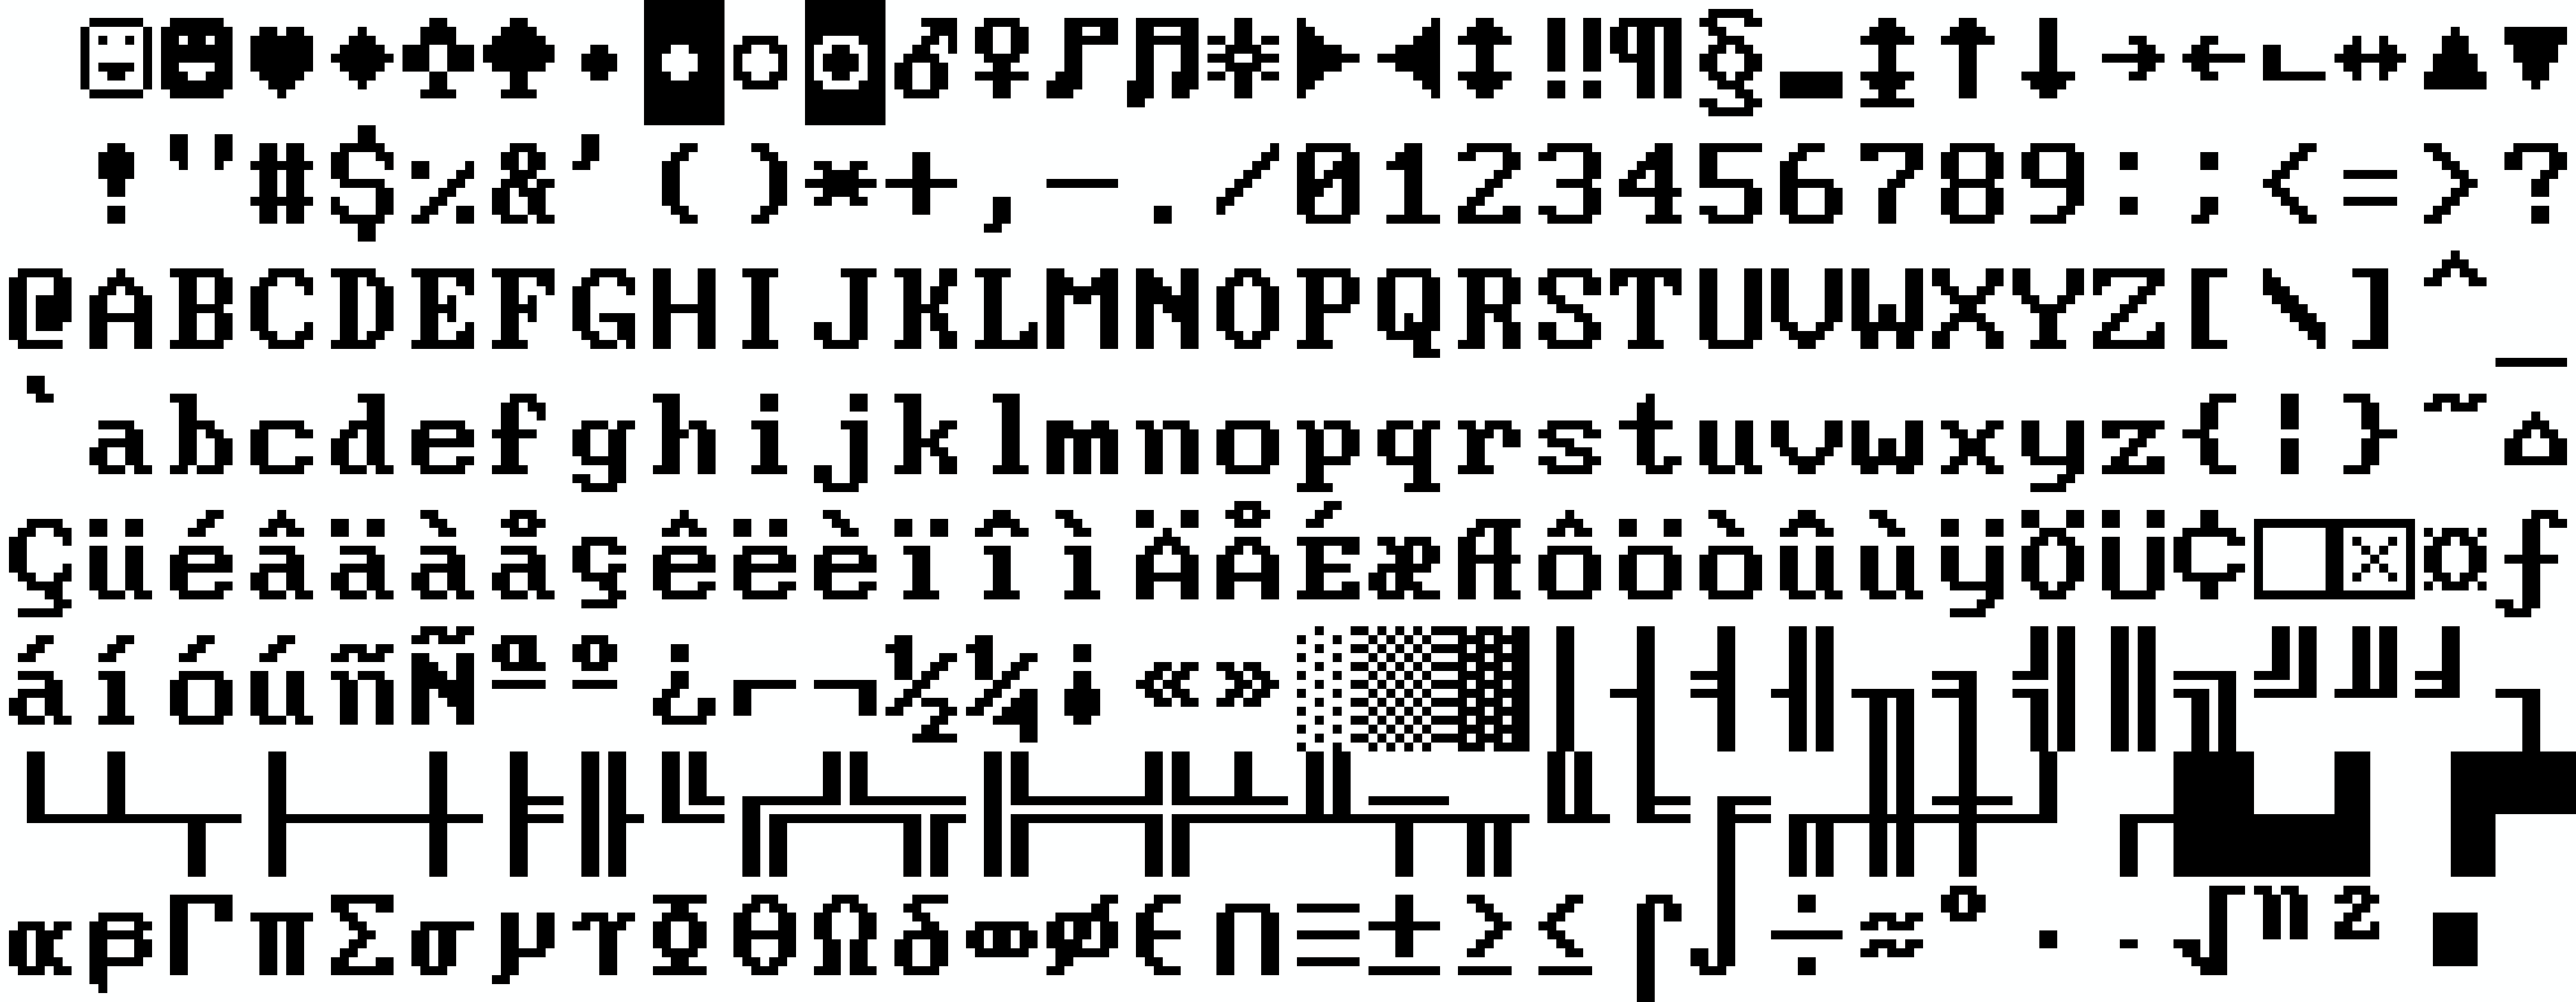
\includegraphics[width=\cpimagew]{mda.png}\end{center}

Character 0x9E (currency symbol) and 0xFA (middle dot) can be accessed with following Lua constants: \emph{MONEY} and \emph{MIDDOT}. See \emph{Lua Globals} > \emph{Constants} section.

\section{Accepted Control Sequences}

\begin{tabularx}{\textwidth}{c X c X}
	\textbf{\large No.} & \textbf{\large Description} & \textbf{\large No.} & \textbf{\large Description}
	\\ \\
	\endhead
	7 & BEL. Emits short tone. & 8 & BS. Moves cursor to left 1 character.
	\\ \\
	9 & TAB. Inserts appropriate horizontal space. Tab size is variable. & 10 & LF. Prints a new line.
	\\ \\
	12 & FF. Clears everything in screen buffer and moves cursor to (1, 1) & 13 & CR. Moves x coordinate of cursor to 1.
	\\ \\
	16 & DLE. Sets foreground colour to the default STDERR colour. & 127 & DEL. Backspace and deletes one character.
	\\ \\
	17 & DC1. Sets foreground colour to 0. (black) & 18 & DC2. Sets foreground colour to 1. (white)
	\\ \\
	19 & DC3. Sets foreground colour to 2. (dim grey) & 20 & DC4. Sets foreground colour to 3. (bright grey)
\end{tabularx}